\documentclass[11pt]{article}
\usepackage[utf8]{inputenc}
\usepackage{amsmath}
\usepackage{amsfonts}
\usepackage[margin=1in]{geometry}
\usepackage{framed}
\usepackage{tikz}
\usepackage{listings}
\usepackage{graphicx}
\usepackage{bbm}
\usepackage{amsthm}
\newtheorem{theorem}{Theorem}
\newtheorem{corollary}{Corollary}[theorem]
\newtheorem{lemma}{Lemma}[theorem]
\newtheorem{assumption}{Assumption}[theorem]
\newtheorem*{remark}{Remark}
\usepackage{amssymb}
\usepackage{mathrsfs}
\usepackage{amsthm}

\usepackage{mathtools}
%\pagenumbering{gobble}
\newcommand{\maxl}{\lambda}
\newcommand{\vlen}{\boldsymbol{h}}
\newcommand{\vint}{\boldsymbol{\omega}}
\newcommand{\vpla}{\boldsymbol{a}}
\newcommand{\innerone}{D_{11}}
\newcommand{\inneronej}{D_{11j}}
\newcommand{\innertwo}{D_{12}}
\newcommand{\innertwoj}{D_{12j}} 
\newcommand{\innerthree}{D_{22}}
\newcommand{\biasone}{B_1}
\newcommand{\biastwo}{B_2}
\newcommand{\biasthree}{B_3}
\newcommand{\Imn}{D}
\newcommand{\Tmn}{T}
\newcommand{\io}{\mathscr{Q}_{p,q}}
\newcommand{\slle}{\hat{\mu}^{LL}_{0j}}
\linespread{1}
\usepackage{bbold}
\usepackage[utf8]{inputenc}
\usepackage{dirtytalk}
\usepackage{float}
\newcommand{\rh}{r\left\lVert \boldsymbol{h}\right\rVert}
\newcommand{\hh}{\left\lVert \boldsymbol{h}\right\rVert}

\newcommand{\bigCI}{\mathrel{\text{\scalebox{1.07}{$\perp\mkern-10mu\perp$}}}}
%\usepackage{cite}
%\usepackage[backend=bibtex,style=verbose-trad2]{biblatex}
%\bibliography{lesson7a1} 
%\bibliographystyle{ieeetr}

\DeclareMathOperator*{\argmin}{arg\,min}
\DeclareUnicodeCharacter{2014}{\dash}
\usepackage{hyperref}
%\usepackage{natbib}
\usepackage{url}

\usepackage[numbers]{natbib}
\bibliographystyle{plainnat} 

%\usepackage{biblatex}
%\addbibresource{prelim.bib}

%\bibliographystyle{plain}

%\DeclareUnicodeCharacter{0027}{\dash}
%\DeclareRobustCommand\dash{%
%  \unskip\nobreak\thinspace\textemdash\allowbreak\thinspace\ignorespaces}
%\bibliography{prelim} 
%\pagestyle{headings}
\allowdisplaybreaks
\newcommand{\Var}{\textrm{Var}}
\newcommand{\Cov}{\textrm{Cov}}
\newcommand{\Br}{\mathcal{B}(\mathbb{R})}

 % \title{Teaching Statement}
 % \author{}
% %\date{Committee Members: Tailen Hsing, Kerby Shedden, Stilian Stoev}
% \date{April 24, 2019}

\begin{document}




\section{Multivariate Model for scores}

Given a model for $Y$, the above gives a relevant functional model. We consider the problem here on how to model the scores $Y$. 

Following Stilian?s formulation, when $d=1$ and $s$ and $t$ are scalar, we consider \begin{align*}
Y(t) &= \int_\mathbb{R}e^{itx}((1 + ix)^{-\nu - 1/2} A1_{\{x > 0\}} + (1 + ix)^{-\nu - 1/2} \overline{A}1_{\{x < 0\}}\tilde{B} (dx)
\end{align*}where $\tilde{B}(dx)$ is $\mathbb{C}^k$-valued Brownian motion with \begin{align*}
\tilde{B}(x) &= \overline{\tilde{B}(-x)} &  \mathbb{E}[\tilde{B}(dx) \tilde{B}(dx)^*] &= \mathbb{I}_k dx
\end{align*}and $A$ is a complex-valued matrix. When $\nu = \nu \mathbb{I}_k$ is a scalar, this above integral gives the covariance \begin{align*}
\mathbb{E}[ Y(t) Y(s)^\top ] &= \int_{\mathbb{R}} e^{i(s-t)x}(1+x^2)^{-\nu-1/2}(AA^*1_{\{x >0\}} + \overline{AA}^*1_{\{x < 0\}})dx.
\end{align*}

\section{The Model}

We consider a covariance model based on the above and derive its validity for any dimension $d$. To do this, we specify a hyperplane that goes through the origin in $d-1$ dimensions that is the plane of reflection of the nonreversibility. When a vector lies on the hyperplane, the model is reversible; when one lies perpendicular to the hyperplane, the model is at its most nonreversible direction. %This formulation is considerably less flexible than the model described above with $\sigma(\theta)$ and $AA^\star(\theta)$.

\subsection{Formulation for general $d$}

Let $ \vlen, \vint$ be vectors in $\mathbb{R}^d$, and let $AA^* = R + iM$ where $R$ is a $k\times k$ real positive definite matrix and $M = \begin{pmatrix} 0 & -m\\  m & 0\end{pmatrix}$ for some $m \in \mathbb{R}$. Let $\vpla$ be a vector in $\mathbb{R}^d$ that describes the plane through the origin for which the non-reversibility is reflected, defined by all $\vint$ such that $\vpla^\top \vint = 0$.

We want to consider the covariance of \begin{align*}
C(\boldsymbol{0}, \boldsymbol{h}) &= \int_{\mathbb{R}^d} e^{i \vint^\top \vlen} (1 +\vint^\top \vint )^{-\nu- \frac{d}{2}} \left(AA^* 1_{\{\vpla^\top \vint > 0\}} + \overline{AA^*} 1_{\{\vpla^\top\vint < 0\}}\right) d\vint% \\
%&=\int_{\mathbb{R}^d} e^{i \vint^\top \vlen }(1 + \vint^\top \vint)^{-\nu- \frac{d}{2}} \left((R + iM)1_{\{\vpla^\top\vint > 0\}} + (R - iM) 1_{\{\vpla^\top\vint < 0\}}\right) d\vint 
\end{align*}
Plugging in $AA^* = R + iM$ gives
\begin{align*}
C(\boldsymbol{0}, \boldsymbol{h})&=\int_{\mathbb{R}^d} e^{i \vint^\top \boldsymbol{h}}(1 + \vint^\top \vint)^{-\nu- \frac{d}{2}} \left(R + iM1_{\{\vpla^\top\vint > 0\}}  - iM1_{\{\vpla^\top\vint < 0\}}\right) d\vint\end{align*}
and by breaking up the integral we have
\begin{align*}
C(\boldsymbol{0}, \boldsymbol{h})%&=\int_{\mathbb{R}^d} (\cos(\vint^\top \boldsymbol{h}) + i\sin(\vint^\top \boldsymbol{h}))(1 + \vint^\top \vint)^{-\nu- \frac{d}{2}} \left(R + iM1_{\{\vint > 0\}}  - iM1_{\{\vint < 0\}}\right) d\vint \\
&=\int_{\mathbb{R}^d}\cos(\vint^\top \boldsymbol{h})(1 + \vint^\top \vint)^{-\nu- \frac{d}{2}} \left(R + iM1_{\{\vpla^\top\vint > 0\}}  - iM1_{\{\vpla^\top\vint < 0\}}\right) d\vint \\
&\ \ \ \ \ \ +i\int_{\mathbb{R}^d}\sin(\vint^\top \boldsymbol{h})(1 + \vint^\top \vint)^{-\nu- \frac{d}{2}} \left(R + iM1_{\{\vpla^\top\vint > 0\}}  - iM1_{\{\vpla^\top\vint < 0\}}\right) d\vint.\end{align*}
Using the even and odd properties of the cosine and sine functions, respectively, gives
\begin{align*}
C(\boldsymbol{0}, \boldsymbol{h})&=R\int_{\mathbb{R}^d}\cos(\vint^\top \boldsymbol{h})(1 + \vint^\top \vint)^{-\nu- \frac{d}{2}} d\vint \\
& \ \ \ \ \ + i^2M\int_{\mathbb{R}^d}\sin(\vint^\top \boldsymbol{h})(1 + \vint^\top \vint)^{-\nu- \frac{d}{2}} \left(1_{\{\vpla^\top\vint > 0\}}  - 1_{\{\vpla^\top\vint < 0\}}\right) d\vint \\
&=R\int_{\mathbb{R}^d}\cos(\vint^\top \boldsymbol{h})(1 + \vint^\top \vint)^{-\nu- \frac{d}{2}} d\vint \\
& \ \ \ \ \ -2M\int_{\vint | \vpla^\top\vint > 0}\sin(\vint^\top \boldsymbol{h})(1 + \vint^\top \vint)^{-\nu- \frac{d}{2}} d\vint .
\end{align*}

When $M$ is the $0$ matrix, each component is Matern, and the above is a simplified version of Gneiting et al (2010) with scale parameter $1$, which is a valid covariance iff $R$ is positive definite and $\nu > 0$. The derivation of the Matern covariance in the univariate case in arbitrary dimension is given in Stein 1999 \textit{Interpolation of Spatial Data}.



 Therefore, in the following, we focus on evaluating the second integral: \begin{align}
\int_{\vint | \vpla^\top\vint > 0}\sin(\vint^\top \boldsymbol{h})(1 + \vint^\top \vint)^{-\nu- \frac{d}{2}} d\vint. \label{toughintegral}
\end{align}We will give the form of the integral, make some remarks and examples, then dive into the proof.

\begin{theorem}
The integral over the half of $\mathbb{R}^d$ specified by \begin{align}
\int_{\vint | \vpla^\top\vint > 0}\sin(\vint^\top \boldsymbol{h})(1 + \vint^\top \vint)^{-\nu- \frac{d}{2}} d\vint. \label{toughintegral}
\end{align} is \begin{align}
&C_{\nu, d}\textrm{sign}(\boldsymbol{a}^\top \boldsymbol{h}) \hh^{\nu}\left(I_\nu(\hh) - \boldsymbol{L}_{-\nu}(\hh)\right) \\
& \ \ \ \ \  -\frac{2\hh^{d/2 - 1}}{\pi}\int_0^\infty \int_{-\infty}^\infty \frac{\sin(|\gamma|(u-r\hh))}{u-r\hh}\frac{\boldsymbol{H}_{d/2 - 1}(u)}{u^{d/2-1}} du (1+ r^2)^{-\nu-d/2} r^{d-1}dr
\end{align}where $I_\nu$ is the modified Bessel function of the first kind, $\boldsymbol{L}_\nu$ is the modified Struve function of the first kind, $\boldsymbol{H}_\nu$ is the Struve function of the first kind, $$C_{\nu,d} = \frac{\pi^{3/2}2^{-d/2}\Gamma(\nu + 1/2)}{\Gamma(\nu + d/2) \cos(\nu\pi)},$$ and $\gamma$ is the cosine of the angle that $\boldsymbol{h}$ makes with the perpendicular vector to $\boldsymbol{a}$.
\end{theorem}

\begin{remark}
I don't know how to do the big integral above in general form. 
\end{remark}

\begin{remark}
When $\gamma=0$, the messy integral disappears. When $\gamma=1$, \begin{align*}
\int_{\vint | \vpla^\top\vint > 0}\sin(\vint^\top \boldsymbol{h})(1 + \vint^\top \vint)^{-\nu- \frac{d}{2}} d\vint =0.
\end{align*}Thus, $\gamma$ controls the strength of reversibility in the cross covariance with respect to direction. For example, if this part of the cross covariance is very reversible with respect to north and south, it will be nonreversible with respect to east and west. Since the symmetric part of the cross covariance is entirely captured with the Mat\'ern, and the cross covariance must satisfy $C_{ij}(h) = C_{ji}(-h)$, the messy integral ensures that this will be the case (I think).
\end{remark}

\begin{remark}
Plot of values of $\textrm{sign}(r)|r|^\nu(I_\nu(r) - \boldsymbol{L}_{-\nu}(r))$ for various $\nu$.

\centering
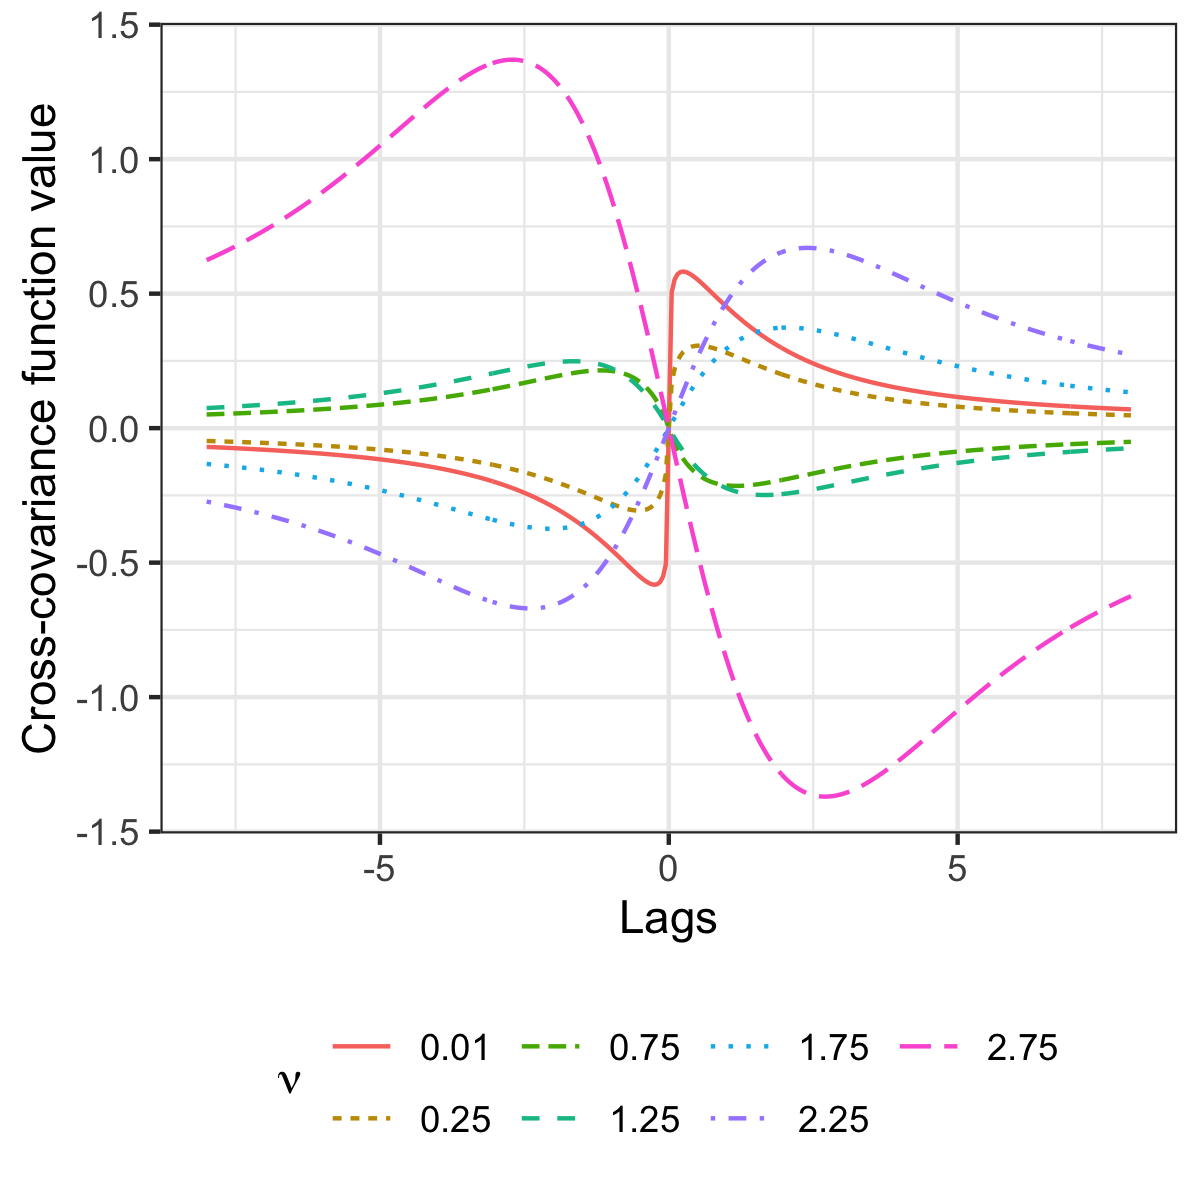
\includegraphics[scale = .15]{../example_fun.png}

\end{remark}

\begin{remark}
The above graph demonstrates the sign of the function. Defining $f_\nu(r) = \textrm{sign}(r)|r|^\nu(I_\nu(r) - \boldsymbol{L}_{-\nu}(r))$, it seems that \begin{align*}
\textrm{sign}(f_\nu(r)) &= \begin{cases} \textrm{sign}(r) & \textrm{ if } \lfloor\nu \rceil \textrm{ is even} \\
-\textrm{sign}(r) & \textrm{ if }\lfloor\nu\rceil \textrm{ is odd} \\ 
\textrm{Does not exist} & \textrm{ if } \nu = 1/2, 3/2, 5/2, \dots \end{cases}
\end{align*}where $ \lfloor x \rceil$ is the rounding function. At $\nu = 1/2, 3/2, \dots$, one could define $f_\nu(r) = 0$ for all $r$, and for these values the only valid cross covariance models of this type are the symmetric Mat\'ern.
\end{remark}


\begin{proof}
We first switch to a form of $d$-dimensional spherical coordinates. A similar approach is done in Stein (1999) page 43. Note that $\sin(\vint^\top \boldsymbol{h}) = \sin(r \left\lVert \boldsymbol{h}\right\rVert \cos(\theta))$ where $\theta$ is the angle between $\vint$ and $\boldsymbol{h}$ and $r = \left\lVert \vint \right\rVert$. Using these coordinates, note that the integral depends only on $r$ and $\theta$, and by integrating the other $d-2$ dimensions with volume transformation $r^{d-1}\sin^{d-2}(\theta)$, we have \begin{align*}
\int_{\vint | \vpla^\top\vint > 0}\sin(\vint^\top \boldsymbol{h})(1 + \vint^\top \vint)^{-\nu- \frac{d}{2}} d\vint&= \textrm{sign}(\boldsymbol{a}^\top \boldsymbol{h})\int_0^\infty \int_{-\pi+c}^c \sin(r\hh\cos(\theta))\sin^{d-2}(\theta) (1+ r^2)^{-\nu-d/2} r^{d-1}d\theta dr
\end{align*}where $c$ is the angle that $\boldsymbol{h}$ makes with $\boldsymbol{a}$. The sign term determines if the angle between $\boldsymbol{h}$ and $\boldsymbol{a}$ is less than or greater than $\pi/2$ degrees. This gives the nice property that the cross covariance at $-\boldsymbol{h} $ is the negative of the cross covariance at $\boldsymbol{h}$. From here we ignore the sign term and assume that it is positive, though we retain it in the final expression.
%Finally, assume without loss of generality that $\boldsymbol{a} = (0,1)^\top$ so that we integrate over the upper half of $\mathbb{R}^2$. See the figure below for a visual representation. Then the integral (\ref{toughintegral}) is \begin{align*}
%&\int_{\vint | \vpla^\top \vint > 0}\sin(\vint^\top \boldsymbol{h})(1 + \vint^\top \vint)^{-\nu- 1} d\vint \\
%&= \int_0^\infty  \int_{-\pi + c}^{c} \sin(r\left\lVert \boldsymbol{h}\right\rVert \cos(\theta)) (1 +r^2)^{- \nu - 1} r d\theta dr. 
% \end{align*}

Now, we complete the proof by the ``formulas in different books" method. The proof relies on the \textit{incomplete} Struve function that modifies the limits of integration for representations of Struve functions. Such functions are studied in detail in \textit{Agrest and Maksimov}. In particular, define \begin{align*}
\boldsymbol{H}_\nu(z) &= \frac{2z^\nu}{A_\nu} \int_0^{\pi/2} \sin(z\cos(\theta)) \sin^{2\nu}(\theta) d\theta, \\
\boldsymbol{H}_\nu(c,z) &= \frac{2z^\nu}{A_\nu} \int_0^{c} \sin(z\cos(\theta)) \sin^{2\nu}(\theta) d\theta
\end{align*}where $A_\nu = 2^\nu\Gamma(\nu + 1/2)\Gamma(1/2)$ as the Struve function and incomplete Struve function, respectively. It is clear that $\boldsymbol{H}_{\nu}(c,z)$ generalizes $\boldsymbol{H}_\nu(z)$ such that $\boldsymbol{H}_\nu(\pi/2, z) = \boldsymbol{H}_\nu(z)$.
% Introducing the incomplete Struve function

By using this definition, we separate the inner integral to have \begin{align*}
&\int_{-\pi+c}^c \sin(r\hh\cos(\theta))\sin^{d-2}(\theta) d\theta = \\
&\ \ \ \ \ \int_{-\pi+c}^0 \sin(r\hh\cos(\theta))\sin^{d-2}(\theta) d\theta + \int_{0}^c \sin(r\hh\cos(\theta))\sin^{d-2}(\theta) d\theta.
%\\\frac{A_{d/2-1}}{2\hh^{d/2-1}}\int_0^\infty (\boldsymbol{H}_{d/2 - 1}(c,r\hh) + (-1)^{d-2} \boldsymbol{H}_{d/2 - 1}(\pi-c, r\hh))  (1+ r^2)^{-\nu-d/2} r^{d/2}dr
\end{align*}Then, focusing on the first integral, we have \begin{align*}
\int_{-\pi+c}^0 \sin(r\hh\cos(\theta))\sin^{d-2}(\theta) d\theta &= (-1)^{d-1}\int_c^\pi \sin(r\hh\cos(w))\sin^{d-2}(w) dw
\end{align*}using the substitution $ w = \theta+\pi$.

Case 1: $d$ is odd. Then  \begin{align}
\int_0^\infty \boldsymbol{H}_{d/2 - 1}(r\hh) (1+ r^2)^{-\nu-d/2} r^{d/2}dr.
\end{align}
So we have \begin{align*}
\int_0^\infty \boldsymbol{H}_{d/2 - 1}(r\hh) (1+ r^2)^{-\nu-d/2} r^{d/2}dr &= \frac{2^{-\nu - d/2}\pi \hh^{\nu+d/2-1}}{\Gamma(\nu + d/2)\cos(\nu\pi)}\left(I_{\nu}(\hh) - \boldsymbol{L}_{-\nu}(\hh)\right)
\end{align*}using 6.814 of I.S. Gradshteyn and I.M. Ryzhik \textit{Tables of Integrals, Series, and Products}. 

Thus, be backpropogating the terms we write \begin{align*}
\frac{A_{d/2-1}}{2\hh^{d/2-1}}2\frac{2^{-\nu - d/2}\pi \hh^{\nu+d/2-1}}{\Gamma(\nu + d/2)\cos(\nu\pi)}\left(I_{\nu}(\hh) - \boldsymbol{L}_{-\nu}(\hh)\right)=C_{\nu,d}\hh^{\nu}\left(I_{\nu}(\hh) - \boldsymbol{L}_{-\nu}(\hh)\right)
\end{align*}where $$C_{\nu,d} = \frac{\pi^{3/2}2^{-\nu - 1}\Gamma(d/2 - 1/2)}{\Gamma(\nu + d/2) \cos(\nu\pi)}.$$Note that this is undefined for $\nu = 1/2, 3/2, \dots$.% but things should work out as one approaches those values. That is, $\cos^{-1}(\nu\pi) \to \infty$ but I believe $\hh^\nu(I_{\nu}(\hh) - \boldsymbol{L}_{-\nu}(\hh))$ goes to infinity as well at the same rate.



Case 2: $d$ is even. We have the same, but with (two times) an adjustment term added


\pagebreak
by separating the integral by $\theta = 0$ and noting \begin{align*}
\int_{-\pi+c}^0 \sin(r\hh\cos(\theta)) \sin^{d-2}(\theta) d\theta &= -\int_{\pi-c}^0 \sin(r\hh\cos(-\ell))\sin^{d-2}(-\ell) d\ell \\
&=(-1)^{d-2} \boldsymbol{H}_{d/2-1}(\pi- c, r\hh) 
\end{align*}since $\sin(-\ell) = -\sin(\ell)$ and $\cos(-\ell) = \cos(\ell)$. \fbox{Justify dropping the $(-1)^{d-1}$} - $\sin^{d-2}(-\ell)$ is a radius in the sphereical coordinates and should be positive.

We are now left to evaluate the general integral of the form \begin{align}
\int_0^\infty \boldsymbol{H}_{d/2 - 1}(c,r\hh) (1+ r^2)^{-\nu-d/2} r^{d/2}dr.\label{test_label}
\end{align}By 3.13 on page 148 of \textit{Agrest and Maksimov}, we have \begin{align}
  \boldsymbol{H}_\nu(c, x) &= \boldsymbol{H}_\nu(x) - \frac{x^\nu}{\pi} \int_{-\infty}^\infty \frac{\sin(|\gamma|(u-x))}{u-x}\frac{\boldsymbol{H}_\nu(u)}{u^\nu} du\label{incomplete_complete}
\end{align}where $\gamma = \cos(c)$. By plugging this into the integral (\ref{test_label}), the first term is \begin{align*}
\int_0^\infty \boldsymbol{H}_{d/2 - 1}(r\hh) (1+ r^2)^{-\nu-d/2} r^{d/2}dr &= \frac{2^{-\nu - d/2}\pi \hh^{\nu+d/2-1}}{\Gamma(\nu + d/2)\cos(\nu\pi)}\left(I_{\nu}(\hh) - \boldsymbol{L}_{-\nu}(\hh)\right)
\end{align*}using 6.814 of I.S. Gradshteyn and I.M. Ryzhik \textit{Tables of Integrals, Series, and Products}. 

Thus, be backpropogating the terms we write the first terms as \begin{align*}
\frac{A_{d/2-1}}{2\hh^{d/2-1}}2\frac{2^{-\nu - d/2}\pi \hh^{\nu+d/2-1}}{\Gamma(\nu + d/2)\cos(\nu\pi)}\left(I_{\nu}(\hh) - \boldsymbol{L}_{-\nu}(\hh)\right)=C_{\nu,d}\hh^{\nu}\left(I_{\nu}(\hh) - \boldsymbol{L}_{-\nu}(\hh)\right)
\end{align*}where $$C_{\nu,d} = \frac{\pi^{3/2}2^{-\nu - 1}\Gamma(d/2 - 1/2)}{\Gamma(\nu + d/2) \cos(\nu\pi)}.$$Note that this is undefined for $\nu = 1/2, 3/2, \dots$ but things should work out as one approaches those values. That is, $\cos^{-1}(\nu\pi) \to \infty$ but I believe $\hh^\nu(I_{\nu}(\hh) - \boldsymbol{L}_{-\nu}(\hh))$ goes to infinity as well at the same rate. This gives the first term in the theorem.

We must now deal with the remaining terms. Note if $\gamma=0$ in (\ref{incomplete_complete}), the second term drops. Furthermore, if $\gamma=1$, we have $c=0$ and $\boldsymbol{H}_{d/2 - 1}(c,r\hh)= 0$, so in that case the entire integral is $0$. These are the two special cases that are easy. I don't really know how to do the general form. 
We write \begin{align*}
\int_0^\infty - \frac{(r\hh)^{d/2 - 1}}{\pi} \int_{-\infty}^\infty \frac{\sin(|\gamma|(u-r\hh))}{u-r\hh}\frac{\boldsymbol{H}_{d/2 - 1}(u)}{u^{d/2-1}} du (1+ r^2)^{-\nu-d/2} r^{d/2}dr  \\
=-\frac{\hh^{d/2 - 1}}{\pi}\int_0^\infty \int_{-\infty}^\infty \frac{\sin(|\gamma|(u-r\hh))}{u-r\hh}\frac{\boldsymbol{H}_{d/2 - 1}(u)}{u^{d/2-1}} du (1+ r^2)^{-\nu-d/2} r^{d-1}dr
\end{align*}and $\gamma=\cos(c)$. Furthermore, combining the terms for $c$ and $\pi-c$ and noting that $|\cos(c)| = |\cos(\pi-c)|$, the entire second term is two times the above.

\pagebreak

Here's one shot. 

Using the sine idenity, we have \begin{align*}
\sin(|\gamma|(u-r\hh)) &= \sin(|\gamma|u)\cos(|\gamma|r\hh) - \cos(|\gamma|u)\sin(|\gamma|r\hh)
\end{align*}we can evaluate \begin{align*}
\int_{-\infty}^\infty \frac{\sin(|\gamma|u)\cos(|\gamma|r\hh)}{u-r\hh}\frac{\boldsymbol{H}_{d/2 - 1}(u)}{u^{d/2-1}} du 
\end{align*}using integration by parts. Namely letting \begin{align*}
w &= \frac{\cos(|\gamma|r\hh)}{u - r\hh} & v &= \sqrt{\pi} \frac{2^{-d/2+1}}{\Gamma(d/2-1/2)} (1 - \gamma^2)^{\nu-3/2}\\
dw &= & dv&=\int_{-\infty}^\infty \frac{\sin(|\gamma|u)}{u^{d/2-1}} \boldsymbol{H}_{d/2-1}(u) du
\end{align*}where one goes from $dv$ to $v$ using (63) of page 107 of tables of integral transforms Vol 1.


\pagebreak

By (1.8) on page 24 (for which $A_\nu =2^\nu \Gamma(\nu+1/2)\Gamma(1/2)$), we have \begin{align*}
 \int_0^{c}  \sin(r\left\lVert \boldsymbol{h}\right\rVert \cos(\theta)) d\theta= \frac{\pi}{2} \boldsymbol{H}_{0}(c, r\left\lVert \boldsymbol{h}\right\rVert)
 \end{align*}where $\boldsymbol{H}_{\nu}(c, z)$ is the incomplete Struve function. Thus, we are left to evaluate \begin{align} 
 \int_0^\infty \frac{\pi}{2}\left(\boldsymbol{H}_{0}(c, r\left\lVert \boldsymbol{h}\right\rVert) + \boldsymbol{H}_{0}(\pi - c, r\left\lVert \boldsymbol{h}\right\rVert)\right) (1+r^2)^{-\nu-1} r dr\label{replace_expression}
 \end{align}
 
% \fbox{What is the value of the integral $\int_0^\infty \boldsymbol{H}_{0}(c, r\left\lVert \boldsymbol{h}\right\rVert) (1 +r^2)^{-\nu - 1} r dr$?}


To evaluate integrals of the type (\ref{replace_expression}), we focus on the integral \begin{align*}
 \int_0^\infty \boldsymbol{H}_{0}(c, r\left\lVert \boldsymbol{h}\right\rVert) (1+r^2)^{-\nu-1} r dr,
\end{align*}which, by substituting, we have \begin{align*}
\int_0^\infty 
\left(\boldsymbol{H}_0(\rh) - \frac{1}{\pi} \int_{\infty}^\infty \frac{\sin(|a|(u-\rh))}{u-\rh}\boldsymbol{H}_0(u) \right) du (1+r^2)^{-\nu-1} r dr
\end{align*}where $a = \cos(c)$. Separating this integral gives \begin{align*}
 \int_0^\infty \boldsymbol{H}_{0}(c, r\left\lVert \boldsymbol{h}\right\rVert) (1+r^2)^{-\nu-1} r dr &= \int_0^\infty\boldsymbol{H}_0(\rh)(1+r^2)^{-\nu - 1}rdr\\ & \ \ \ \ \ \ \ - \frac{1}{\pi}\int_0^\infty\int_{-\infty}^\infty \frac{\sin(|a|(u-\rh))}{u-\rh}\boldsymbol{H}_0(u) du(1+ r^2)^{-\nu-1}rdr
\end{align*}
The first integral has been evaluated above as \begin{align*}
\frac{2^{-\nu -1} \pi \left\lVert \boldsymbol{h}\right\rVert^{\nu}}{\Gamma(\nu+1) \cos(\nu \pi)} \left( I_{\nu }(\left\lVert \boldsymbol{h}\right\rVert) - \boldsymbol{L}_{-\nu} (\left\lVert \boldsymbol{h}\right\rVert)\right),
\end{align*}so we focus on the second integral. 
\end{proof}




\subsection{$d=1$}
 Consider the case $d=1$ where $\omega$ and $h$ are scalars and we have 
  \begin{align*}
\int_{\omega > 0}\sin(\omega h)(1 + \omega^2)^{-\nu- \frac{1}{2}} d\omega
&= \textrm{sign}(h) |h|^{\nu} C_\nu\left(I_{\nu}(|h|) - \boldsymbol{L}_{-\nu} (|h|)\right)
 \end{align*}given on page 332 of Watson: \textit{Theory of Bessel Functions} and $I_\nu$ is the modified Bessel function, $\boldsymbol{L}_\nu$ is the modified Struve function, and $C_\nu = 2^{\nu-1} \sqrt{\pi} \Gamma(-\nu + 1/2)$. Note that this is undefined for $\nu = 1/2, 3/2, \dots$ due to the gamma function, where we have extended the gamma function to the negative nonintegers. As $\nu$ approaches $1/2$, $3/2$, et cetera, it appears that $C_\nu \to \infty$ and $\left(I_{\nu}(|h|) - \boldsymbol{L}_{-\nu} (|h|)\right) \to 0$ at the same rate, resulting in stable values when taking the limit, and one can define those values in the limit.
 
 Also, since the modified Bessel function of the second kind is $K_\nu (z) = \frac{\pi}{2} \frac{I_{-\nu}(z) - I_\nu(z) }{\sin(\nu \pi)}$, and the modified Struve function of the second kind is $M_\nu(z) = \boldsymbol{L}_{\nu}(z) - I_{\nu}(z)$, we have that this is \begin{align*}
 &\textrm{sign}(h) |h|^{\nu} C_\nu\left(I_{-\nu}(|h|) - \frac{2}{\pi}\sin(\nu\pi) K_{\nu}(|h|)- \boldsymbol{L}_{-\nu} (|h|)\right) \\
 &= \textrm{sign}(h) |h|^{\nu} C_\nu\left(- \frac{2}{\pi}\sin(\nu\pi) K_{\nu}(|h|)- M_{-\nu}(|h|) \right)
 \end{align*}because $I_{\nu}(z) = I_{-\nu}(z) -\frac{2}{\pi}\sin(\nu\pi) K_{\nu}(z)$. In the \textit{Theory of Incomplete Cylindrical Functions} $M$ is also denoted as $2F^-$.
 
 %\fbox{What happens when $\nu = 1/2, 3/2, \dots$?}
 
 \subsection{$d=2$}
 
 
 For the 2-dimensional case, we switch to polar coordinates. Note that $\sin(\vint^\top \boldsymbol{h}) = \sin(r \left\lVert \boldsymbol{h}\right\rVert \cos(\theta))$ where $\theta$ is the angle between $\vint$ and $\boldsymbol{h}$ and $r = \left\lVert \vint \right\rVert$. Assume these polar coordinates, and let $c$ be the angle that $\boldsymbol{h}$ makes with the $x$ axis. Finally, assume without loss of generality that $\boldsymbol{a} = (0,1)^\top$ so that we integrate over the upper half of $\mathbb{R}^2$. See the figure below for a visual representation. Then the integral (\ref{toughintegral}) is \begin{align*}
&\int_{\vint | \vpla^\top \vint > 0}\sin(\vint^\top \boldsymbol{h})(1 + \vint^\top \vint)^{-\nu- 1} d\vint \\
&= \int_0^\infty  \int_{-\pi + c}^{c} \sin(r\left\lVert \boldsymbol{h}\right\rVert \cos(\theta)) (1 +r^2)^{- \nu - 1} r d\theta dr. 
 \end{align*}

 
Now, by 12.1.7 of Abramowitz and Stegun \textit{Handbook of Mathematical Functions}, 
\begin{align*}
 \int_0^{\pi/2}  \sin(r\left\lVert \boldsymbol{h}\right\rVert \cos(\theta)) d\theta= \frac{\pi}{2} \boldsymbol{H}_{0}(r\left\lVert \boldsymbol{h}\right\rVert) \end{align*}where $\boldsymbol{H}_\nu$ is the Struve function. One can further see that \begin{align*}
  &\int_{\pi/2}^\pi  \sin(r\left\lVert \boldsymbol{h}\right\rVert \cos(\theta)) d\theta= -\frac{\pi}{2} \boldsymbol{H}_{0}(r\left\lVert \boldsymbol{h}\right\rVert) &   &\int_{-\pi/2}^0  \sin(r\left\lVert \boldsymbol{h}\right\rVert \cos(\theta)) d\theta= \frac{\pi}{2} \boldsymbol{H}_{0}(r\left\lVert \boldsymbol{h}\right\rVert)
 \end{align*}based on properties of $\sin$ and $\cos$. We can now evaluate for two values of $c$:
 
 \begin{enumerate}
\item $c = \pi$: the above integral is $0$, which makes sense since this is the reversible direction as defined. This non-reversible part of the covariance is $0$.
\item $c = \pi/2$: We have \begin{align}
\begin{split} \int_0^\infty  \int_{-\pi/2}^{\pi/2} \sin(r\left\lVert \boldsymbol{h}\right\rVert \cos(\theta)) (1 +r^2)^{- \nu - 1} r d\theta dr&= \int_0^\infty \pi\boldsymbol{H}_0(r\left\lVert \boldsymbol{h}\right\rVert)(1 + r^2)^{-\nu - 1} r dr \\
& =\pi\frac{2^{-\nu -1} \pi \left\lVert \boldsymbol{h}\right\rVert^{\nu}}{\Gamma(\nu+1) \cos(\nu \pi)} \left( I_{\nu }(\left\lVert \boldsymbol{h}\right\rVert) - \boldsymbol{L}_{-\nu} (\left\lVert \boldsymbol{h}\right\rVert)\right)\end{split}\label{complete}
\end{align}by 6.814 of I.S. Gradshteyn and I.M. Ryzhik \textit{Tables of Integrals, Series, and Products}. This gives the non-reversible part perpendicular to the reversible direction. It looks similar to the 1-d case.
 \end{enumerate}
 
 However, this does not work in general because $c\notin \{\pi, \pi/2\}$ necessarily. 


An example of what is going on below. For a fixed $\boldsymbol{h}$, one integrates $\vint$ against the upper half plane. When $\boldsymbol{h}$ is in line with the $x$ axis, the integral is $0$ and the model is reversible across this axis; when $\boldsymbol{h}$ points directly up or down, $c= \pi/2$ and the model is at its most non-reversible direction.

%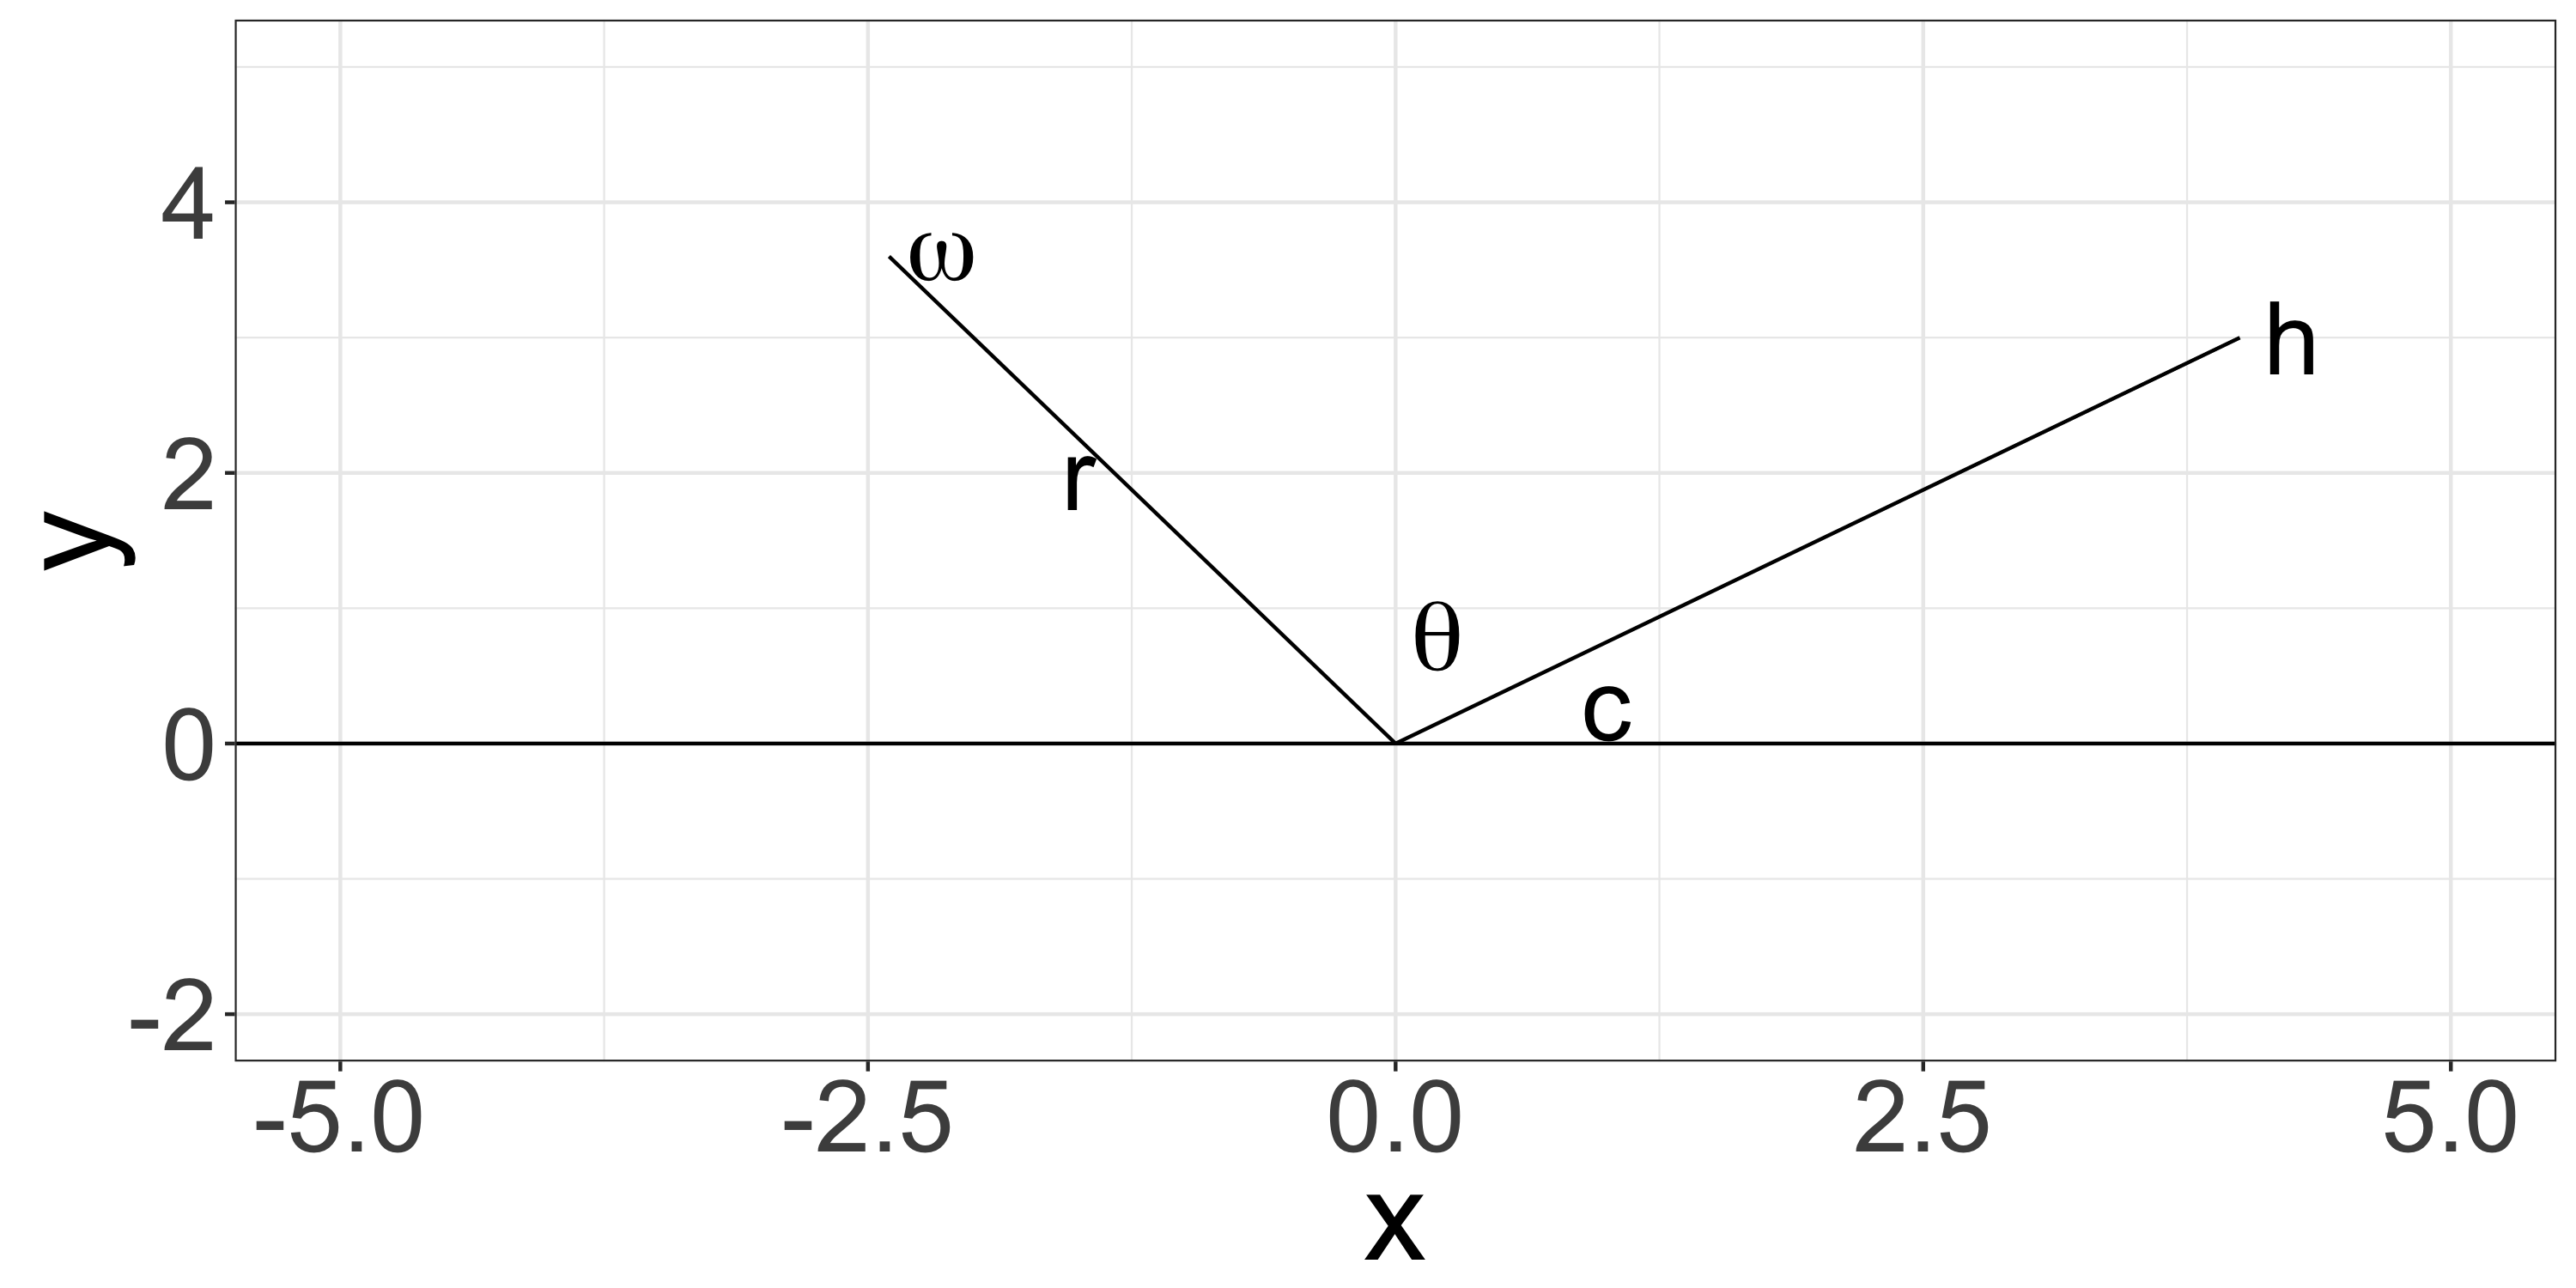
\includegraphics[scale = .1]{angle_plot.png}

\subsubsection{Introduction of Incomplete Cylindrical Functions}

Working with functions with different values of $c$ gives the incomplete cylindrical functions, whose properties are detailed in \textit{Theory of incomplete cylindrical functions and their applications} by M. M. Agrest  M. S. Maksimov. In the following section, the references refer to this book. These functions are given an extra argument for varying values of $c$.

By (1.8) on page 24 (for which $A_\nu =2^\nu \Gamma(\nu+1/2)\Gamma(1/2)$), we have \begin{align*}
 \int_0^{c}  \sin(r\left\lVert \boldsymbol{h}\right\rVert \cos(\theta)) d\theta= \frac{\pi}{2} \boldsymbol{H}_{0}(c, r\left\lVert \boldsymbol{h}\right\rVert)
 \end{align*}where $\boldsymbol{H}_{\nu}(c, z)$ is the incomplete Struve function. Thus, we are left to evaluate \begin{align} 
 \int_0^\infty \frac{\pi}{2}\left(\boldsymbol{H}_{0}(c, r\left\lVert \boldsymbol{h}\right\rVert) + \boldsymbol{H}_{0}(\pi - c, r\left\lVert \boldsymbol{h}\right\rVert)\right) (1+r^2)^{-\nu-1} r dr\label{replace_expression}
 \end{align}
 
% \fbox{What is the value of the integral $\int_0^\infty \boldsymbol{H}_{0}(c, r\left\lVert \boldsymbol{h}\right\rVert) (1 +r^2)^{-\nu - 1} r dr$?}

By 3.13 on page 148 of Theory of incomplete, we have \begin{align*}
  \boldsymbol{H}_\nu(\alpha, x) &= \boldsymbol{H}_\nu(x) - \frac{x^\nu}{\pi} \int_{\infty}^\infty \frac{\sin(|a|(u-x))}{u-x}\frac{\boldsymbol{H}_\nu(u)}{u^\nu} du
\end{align*}where $a = \cos(\alpha)$ and $\alpha \in [0, \pi]$.

To evaluate integrals of the type (\ref{replace_expression}), we focus on the integral \begin{align*}
 \int_0^\infty \boldsymbol{H}_{0}(c, r\left\lVert \boldsymbol{h}\right\rVert) (1+r^2)^{-\nu-1} r dr,
\end{align*}which, by substituting, we have \begin{align*}
\int_0^\infty 
\left(\boldsymbol{H}_0(\rh) - \frac{1}{\pi} \int_{\infty}^\infty \frac{\sin(|a|(u-\rh))}{u-\rh}\boldsymbol{H}_0(u) \right) du (1+r^2)^{-\nu-1} r dr
\end{align*}where $a = \cos(c)$. Separating this integral gives \begin{align*}
 \int_0^\infty \boldsymbol{H}_{0}(c, r\left\lVert \boldsymbol{h}\right\rVert) (1+r^2)^{-\nu-1} r dr &= \int_0^\infty\boldsymbol{H}_0(\rh)(1+r^2)^{-\nu - 1}rdr\\ & \ \ \ \ \ \ \ - \frac{1}{\pi}\int_0^\infty\int_{-\infty}^\infty \frac{\sin(|a|(u-\rh))}{u-\rh}\boldsymbol{H}_0(u) du(1+ r^2)^{-\nu-1}rdr
\end{align*}
The first integral has been evaluated above as \begin{align*}
\frac{2^{-\nu -1} \pi \left\lVert \boldsymbol{h}\right\rVert^{\nu}}{\Gamma(\nu+1) \cos(\nu \pi)} \left( I_{\nu }(\left\lVert \boldsymbol{h}\right\rVert) - \boldsymbol{L}_{-\nu} (\left\lVert \boldsymbol{h}\right\rVert)\right),
\end{align*}so we focus on the second integral. 

% Considering the change of variables $w = |a|( u - \rh)$ and switching the order of integration \hbox{justify}, we have the integral as \begin{align*}
% \int_{-\infty}^\infty \int_{|a|u}^{-\infty} \frac{\sin(w)}{\frac{w}{|a|}} \frac{\boldsymbol{H}_0(u)}{-|a|} dwdu &= \int_{-\infty}^\infty \int_{-\infty}^{|a|u} \frac{\sin(w)}{w} \boldsymbol{H}_0(u) dwdu \\
% &=\int_{-\infty}^\infty(\textrm{Si}(|a|u) - \textrm{Si}(-\infty)) \boldsymbol{H}_0(u) dwdu
% \end{align*}where $\textrm{Si}(x)$ is the sine integral $\int_0^x \sin(t)/t dt$.
%  

\pagebreak


By (5.10) on page 183 and setting $\mu = 2$ and $\nu = 0$, we have $$\int_0^\infty \frac{-\boldsymbol{H}_{0}(c, ax)}{(x^2 + k^2)^{m+1}}x dx = \frac{\pi}{m!} (-1)^{m+1} \left(\frac{d}{dk^2}\right)^{m} F_0^-(c, ak)$$where $$F_0^-(c, ak)=\left\{\frac{I_{0}(c, ak) - \boldsymbol{L}_0(c, ak)}{2}\right\}$$and $I_0(\cdot, \cdot)$ is the incomplete modified Bessel function of the first kind and $\boldsymbol{L}_0(\cdot, \cdot)$ is the incomplete modified Struve function. When $c=  \pi/2$ these reduce to their \say{complete} versions. %This looks close but not exactly right ($m$ is an integer, $\nu$ should be flexible, derivative).

\fbox{\textbf{special case of $\nu=0$}}
Consider the special case where $\nu = 0$. Then, the entire integral is \begin{align*}
&\int_0^\infty\frac{\pi}{2} \left(\boldsymbol{H}_{0}(c, r\left\lVert \boldsymbol{h}\right\rVert) + \boldsymbol{H}_{0}(\pi - c, r\left\lVert \boldsymbol{h}\right\rVert)\right) (1 + r^2)^{-1} r dr \\
\ \ \ \ \ \ \ \ \ &= \frac{\pi}{2} \frac{\pi}{2}\left( I_0(c, \left\lVert \boldsymbol{h}\right\rVert) - \boldsymbol{L}_0(c,\left\lVert \boldsymbol{h}\right\rVert) + I_0(\pi - c, \left\lVert \boldsymbol{h}\right\rVert) - \boldsymbol{L}_0(\pi - c,\left\lVert \boldsymbol{h}\right\rVert)\right)
\end{align*}

When $c = \pi/2$, we reduce to $$\frac{\pi^2}{2} \left( I_0(\left\lVert \boldsymbol{h}\right\rVert) - \boldsymbol{L}_0(\left\lVert \boldsymbol{h}\right\rVert) \right)$$which matches with (\ref{complete}). When $c = \pi$, this reduces to $0$ as expected. 

\fbox{\textbf{different values of $\nu$}}

Assuming that fractional derivatives exist and that we can replace the factorial with the gamma function, we have that , we have \begin{align*}
\int_0^\infty \frac{-\boldsymbol{H}_{0}(c, r \left\lVert \boldsymbol{h}\right\rVert)}{(1 + r^2)^{\nu+1}}r dr=
\frac{\pi}{\Gamma(\nu + 1)} (-1)^{\nu + 1} \left(\frac{d}{d\left\lVert \boldsymbol{h}\right\rVert}\right)^{2\nu} F_0^-(c, \left\lVert \boldsymbol{h}\right\rVert)
\end{align*}Note that $(-1)^{\nu + 1} = \cos(\pi * (\nu+1)) + i\sin(\pi * (\nu+1))$. Consider $\nu= 1/2$. Then this integral is $$\frac{2}{\sqrt{pi}}\pi (\cos(3\pi/2)+i\sin(3\pi/2)) \frac{d}{d \left\lVert \boldsymbol{h}\right\rVert} E_0^+(c,i\left\lVert \boldsymbol{h}\right\rVert).$$Using the derivative defined by $$\frac{\partial E_0^+}{dz} =-E_1^+ + \frac{2i\sin(w)}{\pi}e^{iz\cos(w)}$$(pg 31),we have $$ 2i\sqrt{\pi}\left(- E_1^+(c,i\left\lVert \boldsymbol{h}\right\rVert) + \frac{2 i \sin(c)}{\pi } e^{i\left\lVert \boldsymbol{h}\right\rVert \cos(c)}\right).$$
Using the definition $F_\nu^-(w,z) = \frac{1}{2} e^{i\nu\pi/2}E_\nu^+(w, -iz)$ (pg 25), we have $$2i\sqrt{\pi}\left(- 2 e^{-i \pi/4}F_1^-(c,\left\lVert \boldsymbol{h}\right\rVert) + \frac{2 i \sin(c)}{\pi } e^{i\left\lVert \boldsymbol{h}\right\rVert \cos(c)}\right)$$ which is $$4i\sqrt{\pi}\left(-\frac{1-i}{\sqrt{2}}F_1^-(c,\left\lVert \boldsymbol{h}\right\rVert) + \frac{i \sin(c)}{\pi } e^{i\left\lVert \boldsymbol{h}\right\rVert \cos(c)}\right)$$ which is $$\frac{I_1(c,\left\lVert \boldsymbol{h}\right\rVert) - L_1(c, \left\lVert \boldsymbol{h}\right\rVert)}{2}  - \frac{ \sin(c)}{\pi } e^{i\left\lVert \boldsymbol{h}\right\rVert \cos(c)}.$$ 




%$$\frac{i}{2} \left(- E_1^+(c,i\left\lVert \boldsymbol{h}\right\rVert) + \frac{2 i \sin(c)}{\pi } e^{i\left\lVert \boldsymbol{h}\right\rVert \cos(c)}\right)$$by using pages 31 and 25. This then becomes $$\frac{i}{2} \left(- 2 e^{i \pi/2}F_1^-(c,\left\lVert \boldsymbol{h}\right\rVert) + \frac{2 i \sin(c)}{\pi } e^{i\left\lVert \boldsymbol{h}\right\rVert \cos(c)}\right)$$ which is $$F_1^-(c,\left\lVert \boldsymbol{h}\right\rVert) - \frac{ \sin(c)}{\pi } e^{i\left\lVert \boldsymbol{h}\right\rVert \cos(c)}$$ which is $$\frac{I_1(c,\left\lVert \boldsymbol{h}\right\rVert) - L_1(c, \left\lVert \boldsymbol{h}\right\rVert)}{2}  - \frac{ \sin(c)}{\pi } e^{i\left\lVert \boldsymbol{h}\right\rVert \cos(c)}$$ 
%Consider $\nu = 1$. Then we must compute \begin{align*}\frac{d}{dk^2} F_0^-(c,ak) &= \frac{d}{dk^2} \frac{1}{2} E_0^+(c, iak) \\
%&= \psi_{1}(c, iz) \frac{A_1}{2\pi iz} i^2 \\ 
%&= (iz E_0^+(w, iz) - E_1^+(w, iz)) \frac{A_1}{2\pi z} i\\
%&=
%\end{align*}
%
%Consider $\nu = 1$. Then we must compute \begin{align*}\frac{d}{dk^2} F_0^-(c,ak) &= \frac{d}{dk^2} \frac{1}{2} E_0^+(c, iak) \\
%&= \psi_{1}(c, iz) \frac{A_1}{2\pi iz} i^2 \\ 
%&= (iz E_0^+(w, iz) - E_1^+(w, iz)) \frac{A_1}{2\pi z} i\\
%&= (iz  F_0^-(w, z) -  e^{i \pi/2}F_1^-(w,z)) \frac{A_1}{\pi z} i \\
%&= (-  F_0^-(w, z) -  \frac{i}{z}e^{i \pi/2}F_1^-(w,z)) \frac{2A_1}{\pi } \\
%&= (-  F_0^-(w, z) +  \frac{1}{z}F_1^-(w,z)) \frac{A_1}{\pi } \\
%\end{align*}


% \pagebreak
% 
% 
% 
% Now, this derivative can be evaluated using (1.22) on page 25 and (1.37) on page 27 such that \begin{align*}
% \left(\frac{d}{dk}\right)^{2m} F_0^-(c,ak) &=\frac{1}{2} \left(\frac{d}{dk}\right)^{2m} E_0^+(c, iak)  \\
% &=i^{m} \frac{A_m}{2\pi (ak)^m} \psi_{m}(c, iak)
% \end{align*}
% 
% Therefore, the entire integral is \begin{align*}
%  &\int_0^\infty \frac{\pi}{2}\left(\boldsymbol{H}_{0}(c, r\left\lVert \boldsymbol{h}\right\rVert) - \boldsymbol{H}_{0}(\pi - c, r\left\lVert \boldsymbol{h}\right\rVert)\right) (1+r^2)^{-\nu-1} r dr \\
%  &\ \ \ \ \ \ \ \ \ \ \ = \frac{\pi}{\nu!}(-1)^{\nu + 1} i^\nu \frac{A_\nu}{2\pi \left\lVert \boldsymbol{h}\right\rVert^\nu} \left(-\psi_\nu(c, i\left\lVert \boldsymbol{h}\right\rVert) + \psi_\nu(\pi-c, i\left\lVert \boldsymbol{h}\right\rVert)  \right)\\
%  &\ \ \ \ \ \ \ \ \ \ \ = \frac{\pi}{\nu!}(-1)^{\nu + 1} i^\nu \frac{A_\nu}{\pi \left\lVert \boldsymbol{h}\right\rVert^\nu} \left(\frac{(i\left\lVert \boldsymbol{h}\right\rVert)^\nu}{A_\nu} \left(-\int_0^c e^{-\left\lVert \boldsymbol{h}\right\rVert \cos (t)} \cos^{2\nu} (t) dt + \int_0^{\pi - c} e^{-\left\lVert \boldsymbol{h}\right\rVert \cos (t)} \cos^{2\nu} (t) dt  \right)\right)\\
%  &\ \ \ \ \ \ \ \ \ \ \ = \frac{1}{\nu!} \left(\int_c^{\pi-c} e^{-\left\lVert \boldsymbol{h}\right\rVert \cos (t)} \cos^{2\nu} (t) dt  \right)\\
%   &\ \ \ \ \ \ \ \ \ \ \ = \frac{1}{\nu!} \left(\int_c^{\pi-c} e^{-\left\lVert \boldsymbol{h}\right\rVert \cos (t)} \cos^{2\nu} (t) dt  \right)\\
%  &\ \ \ \ \ \ \ \ \ \ \ = \frac{-2}{\nu!} \frac{A_\nu}{2\left\lVert \boldsymbol{h}\right\rVert^\nu}  \left(E_\nu^-(c,  \left\lVert \boldsymbol{h}\right\rVert) + E_\nu^-(\pi - c,  \left\lVert \boldsymbol{h}\right\rVert) \right)
%  \end{align*}
% 
% The first step comes from using hte derivative. . The second step is using the definition of $\phi$. The third step is cancelling and combining integrals. 
% 
% USE PAGE 31
% 
% By (5.10) on page 183 of \textit{Theory of incomplete cylindrical functions and their applications} and setting $\mu = 2$ and $\nu = 0$, we have $$\int_0^\infty \frac{-\boldsymbol{H}_{0}(c, ax)}{(x^2 + k^2)^{m+1}}x dx = \frac{\pi}{m!} (-1)^{m+1} \left(\frac{d}{dk^2}\right)^{m} F_0^-(c, ak)$$where $$F_0^-(c, ak)=\left\{\frac{I_{0}(c, ak) - \boldsymbol{L}_0(c, ak)}{2}\right\}$$WE NEED AN $i$ in both of theseand $I_0(\cdot, \cdot)$ is the incomplete modified Bessel function orf the first kind and $\boldsymbol{L}_0(\cdot, \cdot)$ is the incomplete modified Struve function. When $m = 0$, this is $$\frac{\pi}{2} (L_0(c, ak) - I_0(c, ak) ).$$ Therefore, the entire integral when $\nu = 0$ is \begin{align*}
%  &\int_0^\infty \frac{\pi}{2}\left(\boldsymbol{H}_{0}(c, r\left\lVert \boldsymbol{h}\right\rVert) + \boldsymbol{H}_{0}(\pi - c, r\left\lVert \boldsymbol{h}\right\rVert)\right) (1+r^2)^{-1} r dr \\
%  &\ \ \ \ \ \ \ \ \ \ \ = \frac{\pi}{4juhnjjnj} \left(L_0(c, \left\lVert \boldsymbol{h}\right\rVert) - I_0(c, \left\lVert \boldsymbol{h}\right\rVert) + L_0(\pi - c, \left\lVert \boldsymbol{h}\right\rVert) -I_0(\pi - c, \left\lVert \boldsymbol{h}\right\rVert)\right)
%  \end{align*}
% This, when $c = \pi/2$ matches the formula for (\ref{complete}) where $\nu = 0$.  Similarly, when $c = \pi$, the above is $0$ as expected. This isn't quite right. (no h)
% 
% 







\end{document}